% LC 受迫振荡电路

\pentry{LC振荡电路\upref{LC}}

当电路中有电阻存在时,由于能量的损耗,电荷和电流的振幅将逐渐减小.
\begin{figure}[ht]
\centering
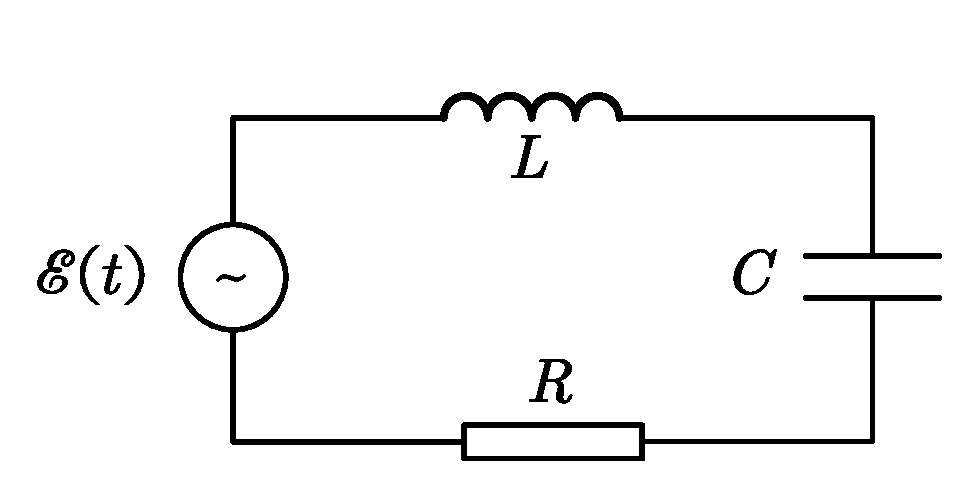
\includegraphics[width=6.5cm]{./figures/EleRes_1.pdf}
\caption{受迫振荡电路} \label{EleRes_fig1}
\end{figure}
如果在电路中加入一个电动势作周期性变化的电源,如\autoref{EleRes_fig1}所示,可以连续不断地供给能量,即可使电流振幅保持不变,这种在外加周期性电动势持续作用下产生的振荡,称为\textbf{受迫振荡(forced oscillation)}.设电源的电动势为$\mathscr{E}=\mathscr{E}_{0} \cos \omega_{\mathrm{d}} t$,则受迫振荡的微分方程可写成
\begin{equation}
L \frac{\mathrm{d}^{2} q}{\mathrm{d} t^{2}}+R \frac{\mathrm{d} q}{\mathrm{d} t}+\frac{q}{C}=\mathscr{E}_{0} \cos \omega_{\mathrm{d}} t
\end{equation}
在稳定状态下其解为
\begin{equation}
q=Q_{0} \cos \left(\omega_{d} t+\phi\right)
\end{equation}
通常我们感兴趣的不是电荷,而是电流的振荡,由上式得
\begin{equation}
\begin{aligned}i&=\frac{\mathrm{d} q}{\mathrm{d} t}=-\omega Q_{0} \sin \left(\omega_{\mathrm{d}} t+\phi\right) \\ &=\omega_{\mathrm{d}} Q_{0} \cos \left(\omega_{\mathrm{d}} t+\phi+\frac{\pi}{2}\right) \\ &=I_{0} \cos \left(\omega_{\mathrm{d}} t+\phi^{\prime}\right)\end{aligned}
\end{equation}
式中
\begin{equation} \label{EleRes_eq1}
I_{0}=\frac{\mathscr{E}_{0}}{\sqrt{R^{2}+\left(\omega_{\mathrm{d}} L-\frac{1}{\omega_{\mathrm{d}} C}\right)^{2}}}
\end{equation}
\begin{equation} \label{EleRes_eq2}
\tan \phi^{\prime}=\frac{\frac{1}{\omega_{\mathrm{d}} C}-\omega_{\mathrm{d}} L}{R}
\end{equation}

可以看到,电流$i$的振荡角频率与电动势的角频率相同,但两者的相位并不相同.

由\autoref{EleRes_eq1}不难看出,当电路满足条件$\omega_{\mathrm{d}} L=\dfrac{1}{\omega_{\mathrm{d}} C}$时,电流将有最大的振幅.从这个条件将$w_\mathrm{d}$解出来,得
\begin{equation}
\omega_{\mathrm{d}}=\sqrt{\frac{1}{L C}}
\end{equation}

这就是说,当外加电动势的频率和自由振荡的的频率相等时,电流的振幅为最大,其值等于$\dfrac{\mathscr{E}_{0}}{R}$,这时,电流和外加电动势之间的相位差$\phi=0$.这种在周期性电动势作用下,电流振幅达到最大值的现象称为\textbf{电共振(electrical resonance)}.收音机中的调谐,就是调节电容器的电容使电路与其某一种频率的无线电信号发生共振,以选取电台.
